\documentclass[fontsize=12pt,toc=bibliography, notitlepage]{scrreprt}

\usepackage[english]{babel}
\usepackage{ucs}
\usepackage[utf8x]{inputenc}
\usepackage[bookmarksopen=true,
			bookmarks=true,
			plainpages=false,
        	pdfpagelabels=true,
			colorlinks=true,
			linkcolor=black,
			citecolor=black,
        	filecolor=black,
        	urlcolor=blue]{hyperref}
\usepackage{graphicx}
\usepackage{float}
\usepackage{listings}
\usepackage{color}
\usepackage{tikz}

\title{Knapsack Genetic Algorithm}
\subtitle{Artificial Intelligence 2}
\author{Fabian Meyer}
\date{\today \\ HTWG Konstanz}

\lstdefinestyle{MyJavaStyle}{
  belowcaptionskip=1\baselineskip,
  breaklines=true,
  frame=single,
  captionpos=b,
  numbers=left,
  xleftmargin=\parindent,
  language=Java,
  showstringspaces=false,
  basicstyle=\footnotesize\ttfamily,
  keywordstyle=\bfseries\color{green!40!black},
  commentstyle=\itshape\color{purple!40!black},
  identifierstyle=\color{blue},
  stringstyle=\color{orange}
}
\lstset{escapechar=@,style=MyJavaStyle}

\newcommand{\refnn}[1]{\ref{#1} \nameref{#1}}

\begin{document}

\maketitle
\tableofcontents

\chapter{Genetic Algorithm}
\label{chap:genetic-algorithm}

\section{Implementation}
\label{sec:implementation}

The Genetic Algorithm is built upon 4 different modules, which influence its behaviour:
\begin{itemize}
	\item \nameref{subsec:parent-selection}
	\item \nameref{subsec:crossover}
	\item \nameref{subsec:selection-of-individuums-to-die}
	\item \nameref{subsec:mutation}
\end{itemize}
Each individuum of a population is a knapsack, which has to fulfil the constraints of a multidimensional knapsack problem (MKP).
The representation of used or unused items is done with arrays of boolean. If the item is included in the knapsack (individuum) the value at the corresponding index is true, else false.

\subsection{Parent Selection}
\label{subsec:parent-selection}
A static breed probability is used to choose how many individuums do breed. A normal distributed random experiment is done n times (n = count of individuums in a population) to determine the number individuums which breed. The outcome of the experiment can only be true or false (lower or higher than the breed probability).
After this the parent individuums are chosen using the \textbf{roulette wheel selection}. Based on their fitness individuums are more less likely to breed. The fitness value is the same as the profit of the individuum. The higher the profit (fitness) of an individuum the higher is the chance of breeding.\\

\subsection{Crossover}
\label{subsec:crossover}
The combination of the genes of the parents is done by uniform crossover. For each gene a coin is tossed. As a result we get an array of boolean (heads = true, tails = false). One child is generated by inheriting all genes of its 'mother', where the coin array shows true, else it inherits the genes of its 'father'. The other child inherits all genes of 'father', where the coins array shows true, else it inherits the genes of its 'mother'.

\subsection{Selection of Individuums to die}
\label{subsec:selection-of-individuums-to-die}
After generating children, we have to select the same amount if individuums from the old population and remove them, so the population keeps the same size. This selection is quite simple, hence it only chooses the individuums with the worst fitness (survival of the fittest, elitism).

\subsection{Mutation}
\label{subsec:mutation}
The mutation is only done on the newly created child individuums. For each child a normal distributed random experiment is done to determine if it mutates or not. If it mutates one gene is randomly chosen and flipped (true -> false, false -> true). After that the rules appliance of the individuum may be broken, so genes are randomly removed until it passes the restrictions. 

\section{Parameter}
\label{sec:parameter}
This implementation of the genetic algorithm (see \refnn{sec:implementation}) is customisable over various parameters. These include:
\begin{itemize}
	\item \nameref{subsec:mutation-probability}
	\item \nameref{subsec:breed-probability}
	\item \nameref{subsec:population-size}
	\item \nameref{subsec:algorithm-duration}
\end{itemize}
These parameters strongly influence the performance of the algorithm related to its speed and quality. In the following the parameters and their influence are discussed.\\
All diagrams show \textbf{problem 0} of the mknapcb1.txt, but the results are applicable for all other problems. The x-axis shows the generation of the population and the y-axis shows the mean profit of the population.

\subsection{Good configuration}
\label{subsec:good-config}

\begin{tabular}{ |l|l| }
	\hline
	Breed probability & 0.8 \\ \hline
	Mutation probability & 0.0001 \\ \hline
	Generation count & 1000 \\ \hline
	Population size & 300 \\ \hline
\end{tabular}
\begin{figure}[H]
	\centering
	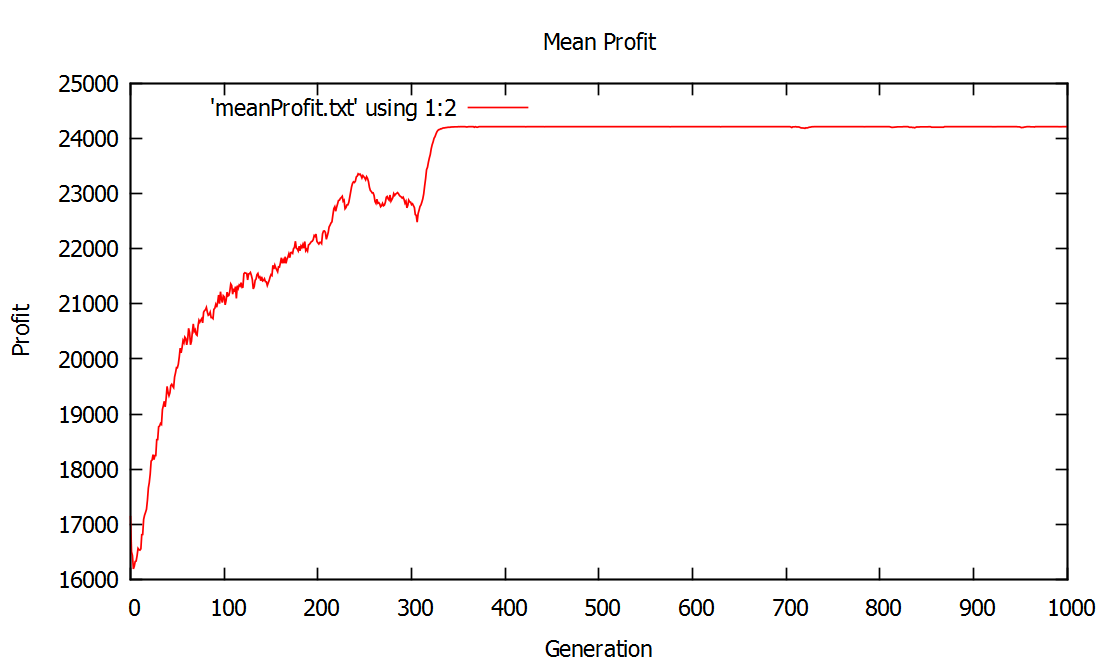
\includegraphics[width=400px]{images/good-config.png}
	\caption{Good configuration}
	\label{fig:good-config}
\end{figure}
Time taken: 13719ms.

\subsection{Mutation Probability}
\label{subsec:mutation-probability}
Multiple tests showed that the mutation probability should be very low (e.g. 0.0001), else the Algorithm never really converges against the optimal solution due to too much randomness.\\
\autoref{fig:mutation-high} shows the following configuration:\\ \\
\begin{tabular}{ |l|l| }
	\hline
	Breed probability & 0.8 \\ \hline
	Mutation probability & 0.2 \\ \hline
	Generation count & 1000 \\ \hline
	Population size & 300 \\ \hline
\end{tabular}
\begin{figure}[H]
	\centering
	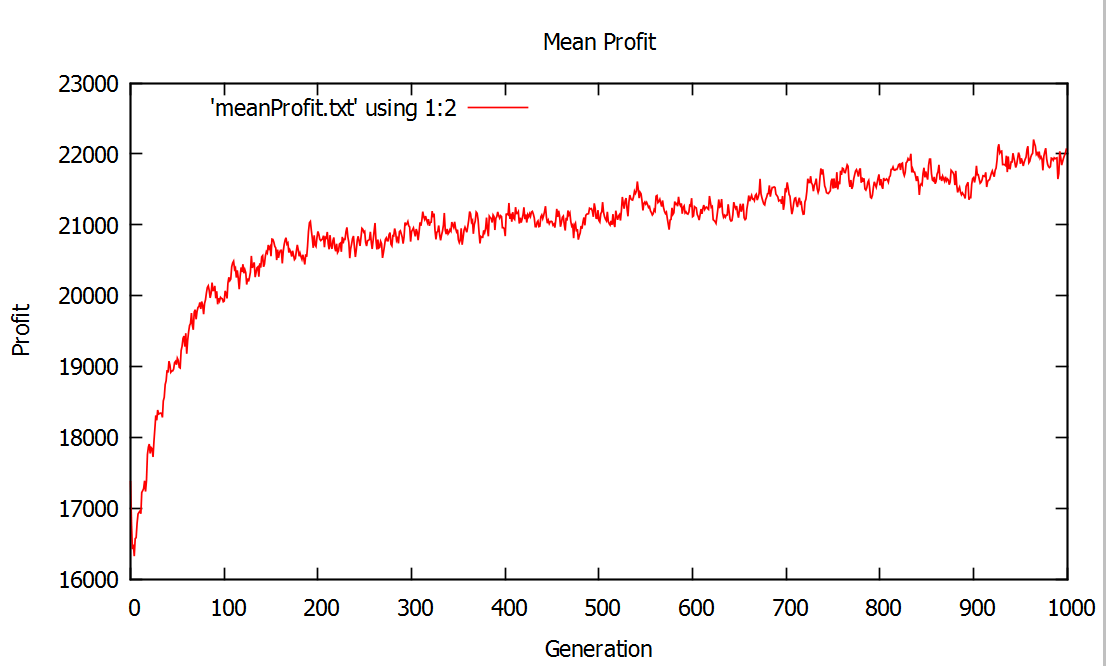
\includegraphics[width=400px]{images/mutation-high.png}
	\caption{High mutation probability}
	\label{fig:mutation-high}
\end{figure}
This figure shows that the algorithm does converge very slowly and there is much noise in the graph. This becomes especially clear if we look at \autoref{fig:good-config}
The configuration of the good configuration is the same as shown in the table above, except that the mutation probability is \textbf{0.0001}. The graph of \autoref{fig:good-config} has much less noise in it and converges much faster than the graph of \autoref{fig:mutation-high}. The low mutation approach also reaches a much higher value in the same amount of generations.

\subsection{Breed Probability}
\label{subsec:breed-probability}
The breed probability should always be a high value (e.g. 0.8), so the population changes a lot. If the probability is too low (e.g. 0.1), the population takes much more generations to improve its overall fitness than with a high probability. Is the probability set too high (e.g. 1.0) , too many individuums of the population are replaced. This leads to also removing the fittest individiuums in the generation and the optimal is never reached.\\
\autoref{fig:breed-low} shows the following configuration:\\ \\
\begin{tabular}{ |l|l| }
	\hline
	Breed probability & 0.1 \\ \hline
	Mutation probability & 0.0001 \\ \hline
	Generation count & 1000 \\ \hline
	Population size & 300 \\ \hline
\end{tabular}
\begin{figure}[H]
	\centering
	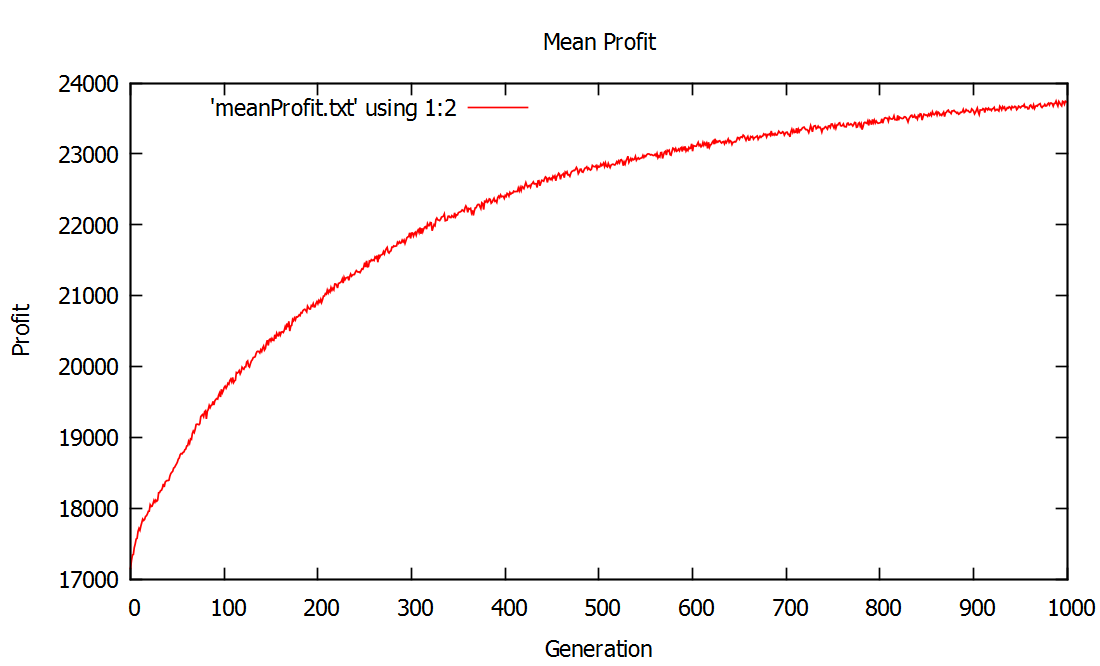
\includegraphics[width=400px]{images/breed-low.png}
	\caption{Low breed probability}
	\label{fig:breed-low}
\end{figure}
The graph of this figure converges very slowly and takes much processing until it reaches the optimum. In comparison to the good configuration shown in \autoref{fig:good-config}, which uses the same parameters as in the table above, but a breed probability of 0.8, the graph of \autoref{fig:breed-low} converges much slower against the optimal solution.\\
\autoref{fig:breed-high} shows the experiment with too high breed probability (1.0).
\begin{figure}[H]
	\centering
	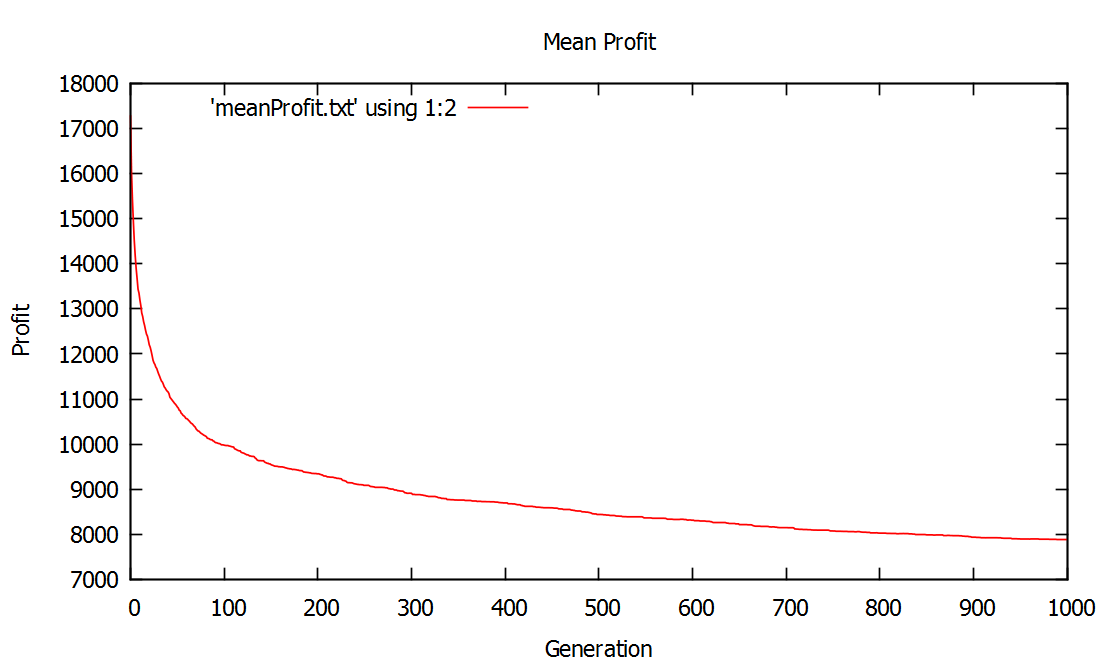
\includegraphics[width=400px]{images/breed-high.png}
	\caption{High breed probability}
	\label{fig:breed-high}
\end{figure}
The overall fitness in the population gets even worse. This is because a breed probability of 1.0 causes all individuums of the population being replaced - even the best. The resulting children may be better or worse than their parents, but after the mutation step it is highly probable that their fitness gets worse. The idea of breeding and mutation is to prevent being stuck at a local optimum. But if the algorithm also removes the best individuums, the overall fitness decreases.

\subsection{Population Size}
\label{subsec:population-size}
With a high population size there is plenty of gene diversity in the population, but the algorithm takes longer to calculate. A low population size leads to less diversity. If it is too low, the algorithm gets stuck in a local optimum, because some genes are missing in the population.\\
\autoref{fig:population-high} shows the following configuration: \\ \\
\begin{tabular}{ |l|l| }
	\hline
	Breed probability & 0.8 \\ \hline
	Mutation probability & 0.0001 \\ \hline
	Generation count & 1000 \\ \hline
	Population size & 1000 \\ \hline
\end{tabular}
\begin{figure}[H]
	\centering
	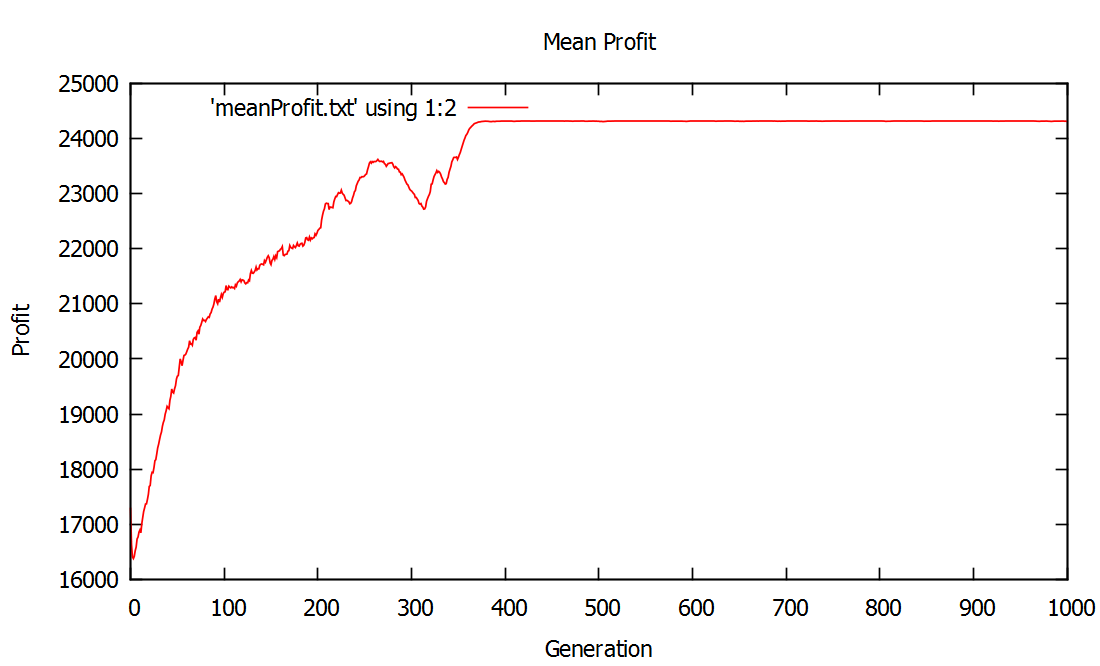
\includegraphics[width=400px]{images/population-high.png}
	\caption{High population size}
	\label{fig:population-high}
\end{figure}
This run performs equally as good as the good solution (see \autoref{fig:good-config}), but it takes way more processing time. Instead of 13719ms of the good configuration (see \refnn{sec:good-config}), this one has taken 154519ms, which is 11 times more.\\
An approach with a very low population size (10) is shown in \autoref{fig:population-low}.
\begin{figure}[H]
	\centering
	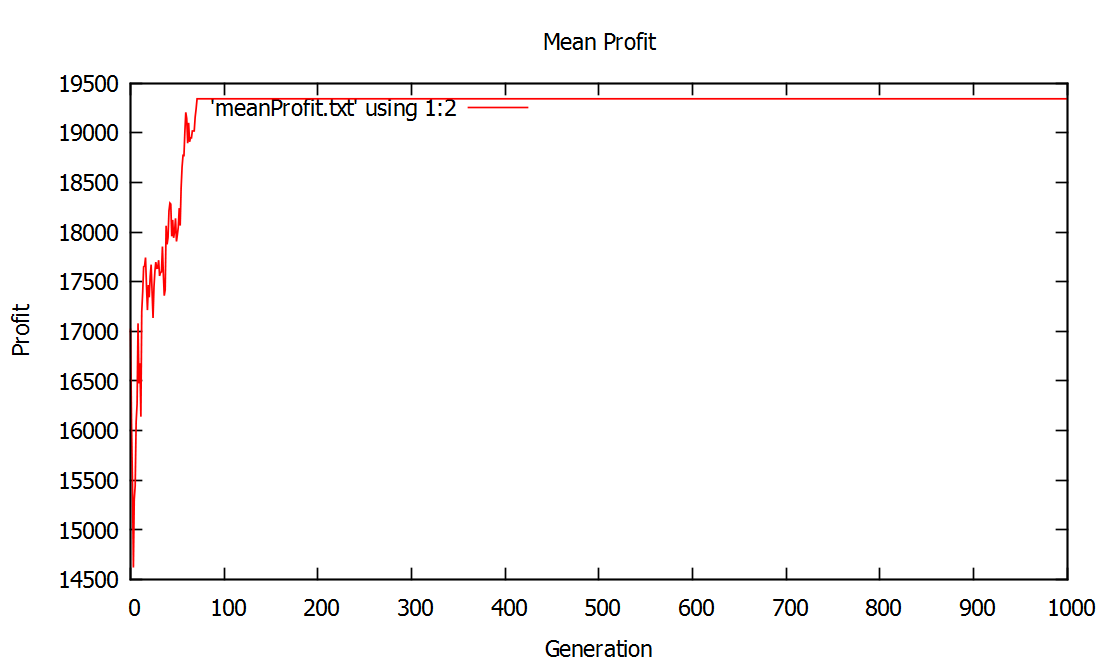
\includegraphics[width=400px]{images/population-low.png}
	\caption{Low population size}
	\label{fig:population-low}
\end{figure}
The graph of \autoref{fig:population-low} converges really fast, due to less individuums to optimize. But the population gets stuck at a local optimum. The the graph of \autoref{fig:good-config} converges against about 24000 while \autoref{fig:population-low} converges against about 19400. This approach leads to a suboptimal solution.

\subsection{Generation Count / Duration}
\label{subsec:algorithm-duration}
How high the generation count or duration should be set depends on how much time you are able to wait for the results. More generations lead to a better or optimal solution. Too less generations can lead to a graph that does not reach the optimum. \\
\autoref{fig:generation-low} shows a low generation approach with the following configuration: \\ \\
\begin{tabular}{ |l|l| }
	\hline
	Breed probability & 0.8 \\ \hline
	Mutation probability & 0.0001 \\ \hline
	Generation count & 100 \\ \hline
	Population size & 300 \\ \hline
\end{tabular}
\begin{figure}[H]
	\centering
	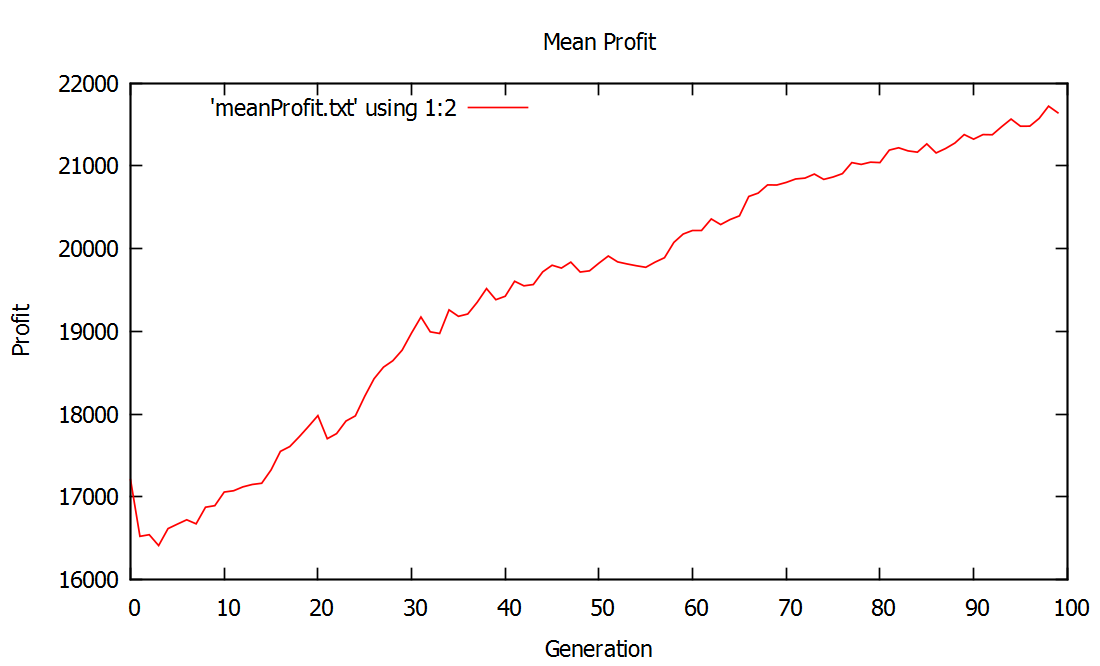
\includegraphics[width=400px]{images/generation-low.png}
	\caption{Low generation count}
	\label{fig:generation-low}
\end{figure}
In comparison to \autoref{fig:good-config} this one does not even nearly reach the optimal value. The graph of \autoref{fig:generation-low} does not converge and shows increasing behaviour. The conclusion is that the solution can be better, if we process more generations.

\begin{thebibliography}{999}

\end{thebibliography}

\cleardoublepage
\addcontentsline{toc}{chapter}{\listfigurename}
\listoffigures

\end{document}